% Template for IGARSS-2020 paper; to be used with:
%          spconf.sty  - LaTeX style file, and
%          IEEEbib.bst - IEEE bibliography style file.
% --------------------------------------------------------------------------
\documentclass{article}
\usepackage{spconf,amsmath,epsfig}
\usepackage{subcaption}
\usepackage{multirow}
% Example definitions.
% --------------------
\def\x{{\mathbf x}}
\def\L{{\cal L}}

% Title.
% ------
\title{A PARSIMONIOUS NEURAL NETWORK FOR THE CLASSIFICATION OF MODIS TIME-SERIES}
%
% Single address.
% ---------------
\name{T.L. Grobler$^{\dagger}$, W. Kleynhans$^{\star}$ and B.P. Salmon$^{\ddagger}$}
\address{$\dagger$Dept of Mathematical Sciences, Computer Science Division, Stellenbosch University,\\ Private Bag X1, 7602 Matieland, South Africa\\
$\star$Department of Electrical, Electronic and Computer Engineering University of Pretoria,\\
Pretoria 0002, South Africa\\
${\ddagger}$School of Engineering, University of Tasmania,
Hobart, TAS 7001, Australia}
%
% For example:
% ------------
%\address{School\\
%	Department\\
%	Address}
%
% Two addresses (uncomment and modify for two-address case).
% ----------------------------------------------------------
%\twoauthors
%  {A. Author-one, B. Author-two\sthanks{Thanks to XYZ agency for funding.}}
%	{School A-B\\
%	Department A-B\\
%	Address A-B}
%  {C. Author-three, D. Author-four\sthanks{The fourth author performed the work
%	while at ...}}
%	{School C-D\\
%	Department C-D\\
%	Address C-D}
%
\begin{document}
%\ninept
%
\maketitle
%
\begin{abstract}
The Gramien Angular Field (GMF) transform encodes time-series into images so that image based classification approaches can be exploited to perform time-series classification. Settlement expansion is one of the most pervasive forms of landcover change in sub-saharan Africa. In this paper, we show that the GAF transform outperforms the conventional techniques we compared against when it is employed in conjunction with Moderate Resolution Imaging Spectroradiometer (MODIS) time-series to detect settlement expansion in the Gauteng province of South Africa.   
\end{abstract}
%
\begin{keywords}
Moderate Resolution Imaging Spetroradiometer, Gramian Angular Fields, landcover classification and change detection, settlement expansion
\end{keywords}
%
\section{Introduction}
\label{sec:intro}
A Convolutional Neural Network (CNN) is a special kind of neural network which is capable of extracting its own features. To achieve this, CNNs use trainable two dimensional convolutional filters in its architecture. CNNs have had great success in performing land-cover classification of high resolution imagery. The CNNs that are used for land-cover classification of high resolution imagery usually make use of convolutional filters along the spatial and spectral dimension.

Temporal CNNs (TCNs) are convolutional networks that
exploit the temporal dimension of multi-variate time-series. TCNs differ from normal CNNs in that convolutional filters are also applied along the temporal axis. Recent studies have shown that TCNs can be very effective when used for the classification of remote sensing time-series. 

In xx, fully fledge multiple channel TCNs are used for remote sensing time-series classification. In contrast, in this paper we investigate how effective a parsimonous single channel TCN can be when employed for time-series classification. To state it differently, we are in fact not trying to create a TCN at all, but rater a parsimonioun feed forward neural network which makes use of convolutions to efficiently process remote sensing time-series. To summarize, in this paper we show that convolutional filters can be effectively applied to remote sensing time-series due to its multi-spectral and seasonal nature to create a highly parsimonious feed forward network (see Fig.~\ref{fig:mv_series}).   

\section{Data Description}
\label{sec:data}
In this paper we make use of MCD43A4 MODIS time-series. We use the first seven MODIS bands. The spatial resolution of MODIS is 500~m by 500~m. The temporal cadence of the time-series is every eight days (45 observations a year). The study area is in Gauteng, South Africa and is approximately 230~km$^2$. The time-period considered was between January 2001 and March 2009. We consider two landcover types in this paper, namely vegetation ($v$) and settlement ($s$) pixels. A pixel was classified as beign vegetation if it contained more than 90\% vegetation. If the pixel contained more than 50\% buildings it was classified as a settlement pixel. 
The MODIS time-series dataset consists of 925 pixels, of which 592 pixels were vegetation pixels and 333 pixels were settlement. Pixels were selected by visually inspecting two high-resolution Syst\`{e}me Probatoried d'Observation de la Terra (SPOT) images from 2001 and 2009. Only pixels that according to the SPOT images did not change were selected. A random vegetation pixel from this dataset is depicted in Fig~\ref{fig:mv_series}. 

\begin{figure}
  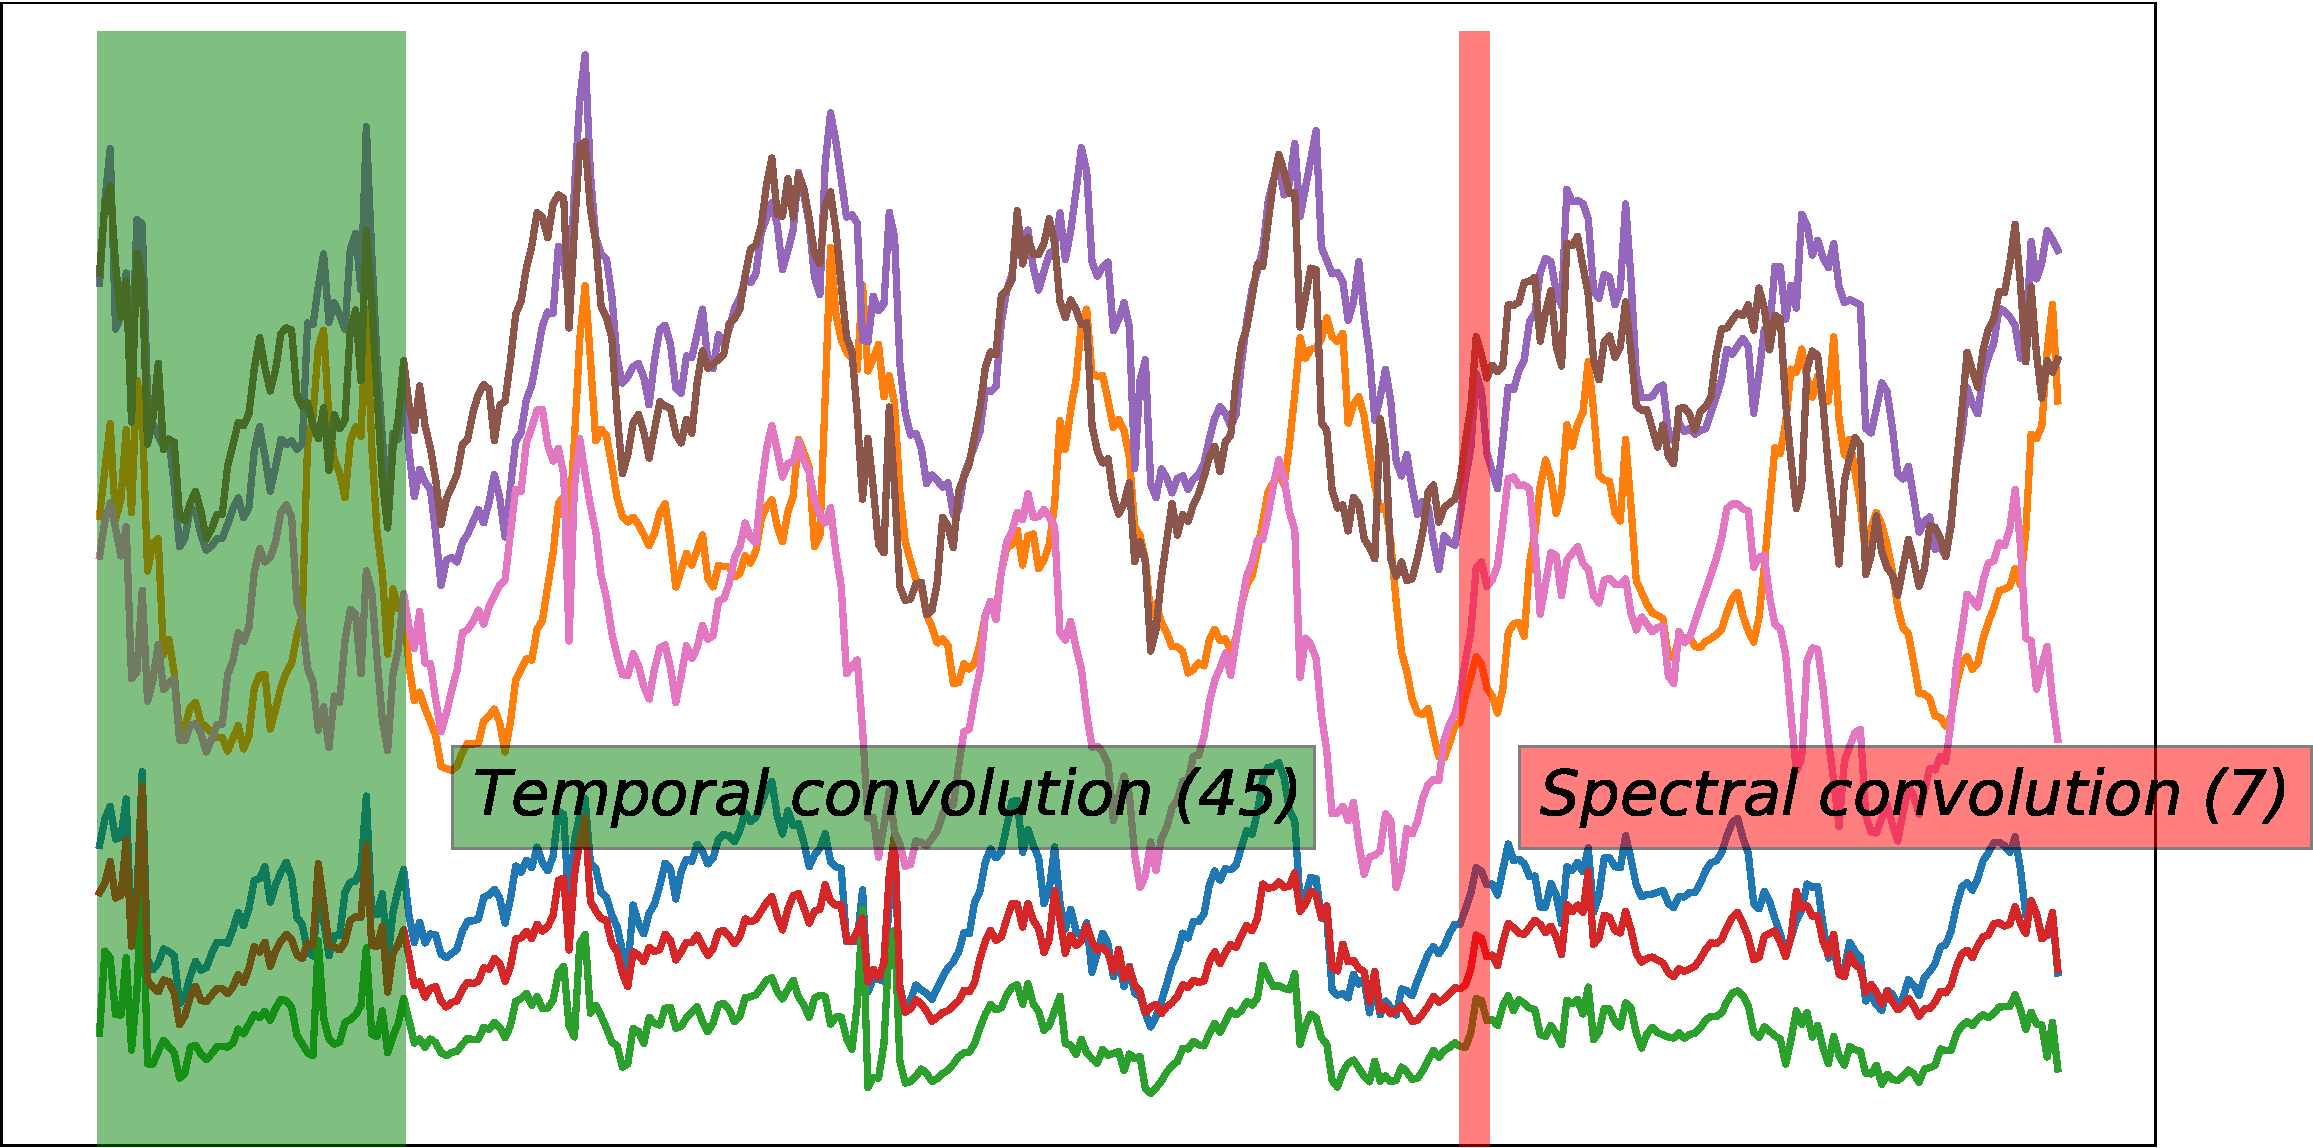
\includegraphics[width=0.48\textwidth]{time_series-crop.pdf}
  \caption{A random vegetation pixel from the MODIS dataset we considered in this paper. A MODIS pixel is a multi-variate time-series. The multi-spectral time-series can be combined into a single time-series by employing a convolutional filter along the spectral domain of size 7. The time-series are highly sinusoidal in nature (a period of 45 observations). A convolutional filter along the temporal domain of size 45 (and a step size of 45) can in principal be used to effectively capture the saliant yearly information contained within the multi-variate time-series.}
 \label{fig:mv_series} 
 \end{figure}
 
 \section{Convolutional Neural Netwrok}
 A nerual network is a graph like structure whose nodes are known as neurons. A neural network can consist of multiple layers, an input layer, multiple hidden layers and an output layer. Each layer's nodes is connected to all the other nodes of the next layer. To emphasize this, we normally refer to the layers of a neural network as being fully connected layers. One of the major uses of neural networks is to perform classification. When used for classification we feed into it a variaty of classification features. It then generates a classification label. Associated with each edge that conncects two neurons is a weight and a bias term. The weight represents the signal strength of the information beigh passed on via the edge in question. Associated with each node is an activation function, which determines if the information should be passed forward or not. At a node the weighted inputs are summed and then passed through the activation function. A convolutional neural network is nothing more than a specific kind of neural network. In addition to containing fully connected layers it also contains convolutional and pooling layers. The convolutional layer simply consist of a convolutional filter which is slided over the input layer's nodes. The degree of sliding is determined by the step size. The convolutional filter is nothing more than a bunch of weights that are multiplied with the input node values. The weighted values are then passed to an output node. The output node then processes the information just as before. The main difference then between a fully connected layer and a convolutional layer is that not all of the input and output nodes of a layer need to be connected with one another. Moreover, the weights are re-used and do not differ for multiple output nodes. This dramatically reduces the number of parameters needed by convolutional layers. The pooling layers are used for downsampling and als involves using a convolutional filter which is slided accros a layer's input nodes. In this case instead of weighing the inputs you simply take that average or the max value of the inputs and pass that value forward to the next layer. As we have said before a TCN is simply an CNN that employs convolutional filters along the temporal domain. 
 
\section{Methodology}
\label{sec:exp}
In this section we describe the experiment we conducted to show that one can construct a parsimonious neural network for remote sensing time-series classification by employing convolutional filters. We start the section by introducing the benchmarking architecture we compared against to show that our architecture does in fact work. We then introduce our parsimonious architecture. We then describe how we trained and evaluated the models we obtained from the two architectures. 

\subsection{Architecture A}
Our benchmarking arrchitecture is depicted in the left panel of Fig.~\ref{}. In the case of Architecture A all of the recorded values are regarded as features. All data-points are simply passed into a sigmoid activation function. So no data reduction is performed. It is, therefore,  nothing more than a logistic regression classifier.
The total number of trainable parameters in architecture A is 2577.

\subsection{Architecture B}
Architecture B makes use of convolutional filters and is depicted in the left panel of Fig.\ref{}. The data is first passed throug a spectral convolutional layer which combines the multivariate time-series into a single time-series. Note that the output from the spectral convolutional layer is reshaped so that any superfluous dimensions are first removed at this point iun time before continuing. The single time-series is then passed through a temporal convolutional layer with a kernal size of 45. The step size of the temporal layer is also 45. The convolutional layer therefore returns eight values per pixel. The eight values can be interpreted as the yearly sailiant information that is contained within the time-series. We used the tanh activation function in all the aformentioned layers. We then flatten the data, again this removes any superfluous dimensions that remain. The data is then passed through a fully connected layer. And finally the data is passed through a sigmoid layer. The normalized weights for a random trained model of architecture B is depicted in Fig.~\ref{}. The total number of trainable parameters in architecture B is 135.
     

\subsection{Training, Evaluation and Hyperparameters}

We used a standard training, validation and test set split. Our training set contained 50\% of the data, our validation set contained 25\% of the data and our test set contained 25\% of the data. The experiment was repeated 100 times to investigate the stability of the results. During each run a different subset of the data was used for training, testing and validation. We used a batch size of ten. The model obtained after ten epochs was used for evaluation purposes (the validation results indicated that a good model was found after about ten epochs). The Adam optimizer was used and a learning rate of $10^{-2}$ was chosen. We used L2 regularization to avoid overfitting (our regularization constant was set to $10^{-3}$).    


\section{Results}
\label{sec:results}
The confusion matrices associated with the experiments conducted in Section~\ref{sec:exp} are reported in Table~\ref{tab:cm}. The diagonal entries of the confusion matrix report the per class accuracy of the experiments in Section~\ref{sec:exp}. Architecture B uses roughly 19 times less parameters than Architecture A, but achieves a similar classification accuracy. We can therefore conclude that for the case study presented  convolutional filters can be used to drastically reduce the number of parameters in the feedforward network that is used the classify the dataset in Section~\ref{}. 

\section{Conclusion}
In this paper we investigated whether convolutional filters could be used to decrease the number of parameters in a feed forward neural netwrok that is used for the classification of remote sesning time-series. We presented a possible architecture to acieve this (see right panel of Fig~\ref{}). This architecture
contains a spectral convolutional filter that combines the different bands into one band and a temporal filter that is able to extract the salient information contained within every year of the data. If we compare the classification results of this architecture with a simple logistic sigmoid classifier we find that for the case study presented the two classifiers perfrom similarly. This implies that for the case study we presented it is indeed possible to reduce the number of parameters in a feedforward neural network by employing convolutional filters. Whether this generalizes to other datasets will be investigated in a future work.  

\label{sec:results}
\begin{table}
\begin{tabular}{ |l|c c c| }
\hline
%\multicolumn{3}{ |c| }{Team sheet} \\
& & s & v\\
\hline
\multirow{2}{*}{Architecture A} & \emph{s} & 96.58\%$\pm$4.41&3.42\%\\
& \emph{v}& 0.68\%& 99.32\%$\pm$1.49\\
\hline
\multirow{2}{*}{Architecture B} & \emph{s} & 96.16\%$\pm$3.83&3.84\%\\
& \emph{v}& 2.04\%& 97.96\%$\pm$1.49\\
%Goalkeeper & GK & Paul Robinson \\ \hline
%\multirow{4}{*}{Defenders} & LB & Lucas Radebe \\
% & DC & Michael Duburry \\
% & DC & Dominic Matteo \\
% & RB & Didier Domi \\ \hline
%\multirow{3}{*}{Midfielders} & MC & David Batty \\
% & MC & Eirik Bakke \\
% & MC & Jody Morris \\ \hline
%Forward & FW & Jamie McMaster \\ \hline
%\multirow{2}{*}{Strikers} & ST & Alan Smith \\
% & ST & Mark Viduka \\
\hline
\end{tabular}
\caption{The confusion matrices associated with the experiments described in Section~\ref{sec:exp}. The labels v and s are shorthand for vegetation and settlement, respectively. The labels that are not italicized represent the true labels, while the italicized labels represent the predicted labels.}
\label{tab:cm}
\end{table}

%Given this background, let us list the  contributions that we make in this paper: 
%\begin{itemize}
% \item Our indepenent study corroborates the study made by Dias et al, i.e. we have confirmed that the GAF transform is a usefull encoding scheme that can be used for pixel-based land cover classification. 
% \item We show that the GAF transform can be utilized for detecting settlement expasion.
% \item We show that the GAF transform can not only be used for pixel based land cover classification, but also for detecting land cover change.
% \item We show that is the classification problem at hand is seperable enough
%\end{itemize}




% Below is an example of how to insert images. Delete the ``\vspace'' line,
% uncomment the preceding line ``\centerline...'' and replace ``imageX.ps''
% with a suitable PostScript file name.
% -------------------------------------------------------------------------

\begin{figure*}
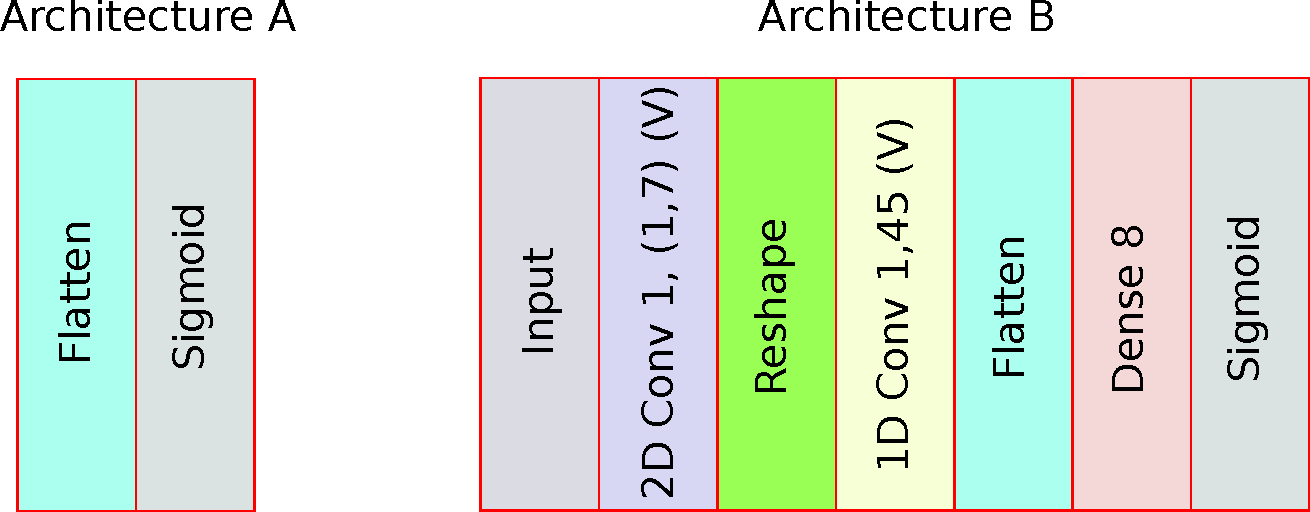
\includegraphics[width=0.9\textwidth]{Architectures.pdf} 
\caption{The two architectures we used in this paper are presented in this figure. The benchmarking architecture is presented in the left panel and is referred to as architecture A. The novel architecture is presented in the right panel and is referred to as architecture B. Architecture A represents a basic sigmoid classifier that takes in all observaed values. Architecture B first applies a convolutional filter along the spectral domain followed by a temporal filter along the temporal domain. The output of the temporal convolutional layer is passed to a fully connected layer. The output of the dense layer is passed to a sigmoid output layer. The shorthand notation $x, y~(\textrm{V})$ used to describe the convolutional layers should be interpreted as follows: $x$ refers the number of output channels, $y$ refers to the kernal size to use (if a tuple then it implies that a multi-dimensional kernal should be used), while (V) indicates that valid padding was used. A step size of one and 45 were respectively used for the spectral and the temporal layer. The eight label in the dense layer block indicates the number of nodes it consisted of. The tanh activation function was used in all convolutional and hidden layers. The hyperparameters used to train these two architectures are discussed in Section~\ref{}. The reshape and Flatten layers get rid of any superfluous dimensions present in the data. Architecture A uses 2577 parameters, while architecture B requires only 135 parameters. The normalized weights associated with architecture B for a randomly trained model of architecture B is presented in Fig~\ref{}. The performance of the two architectures are similar even though architecture A uses roughly 19 times more parameters than architecture B (see Table~\ref{}).}
\label{fig:ach}

\end{figure*}

\begin{figure*}
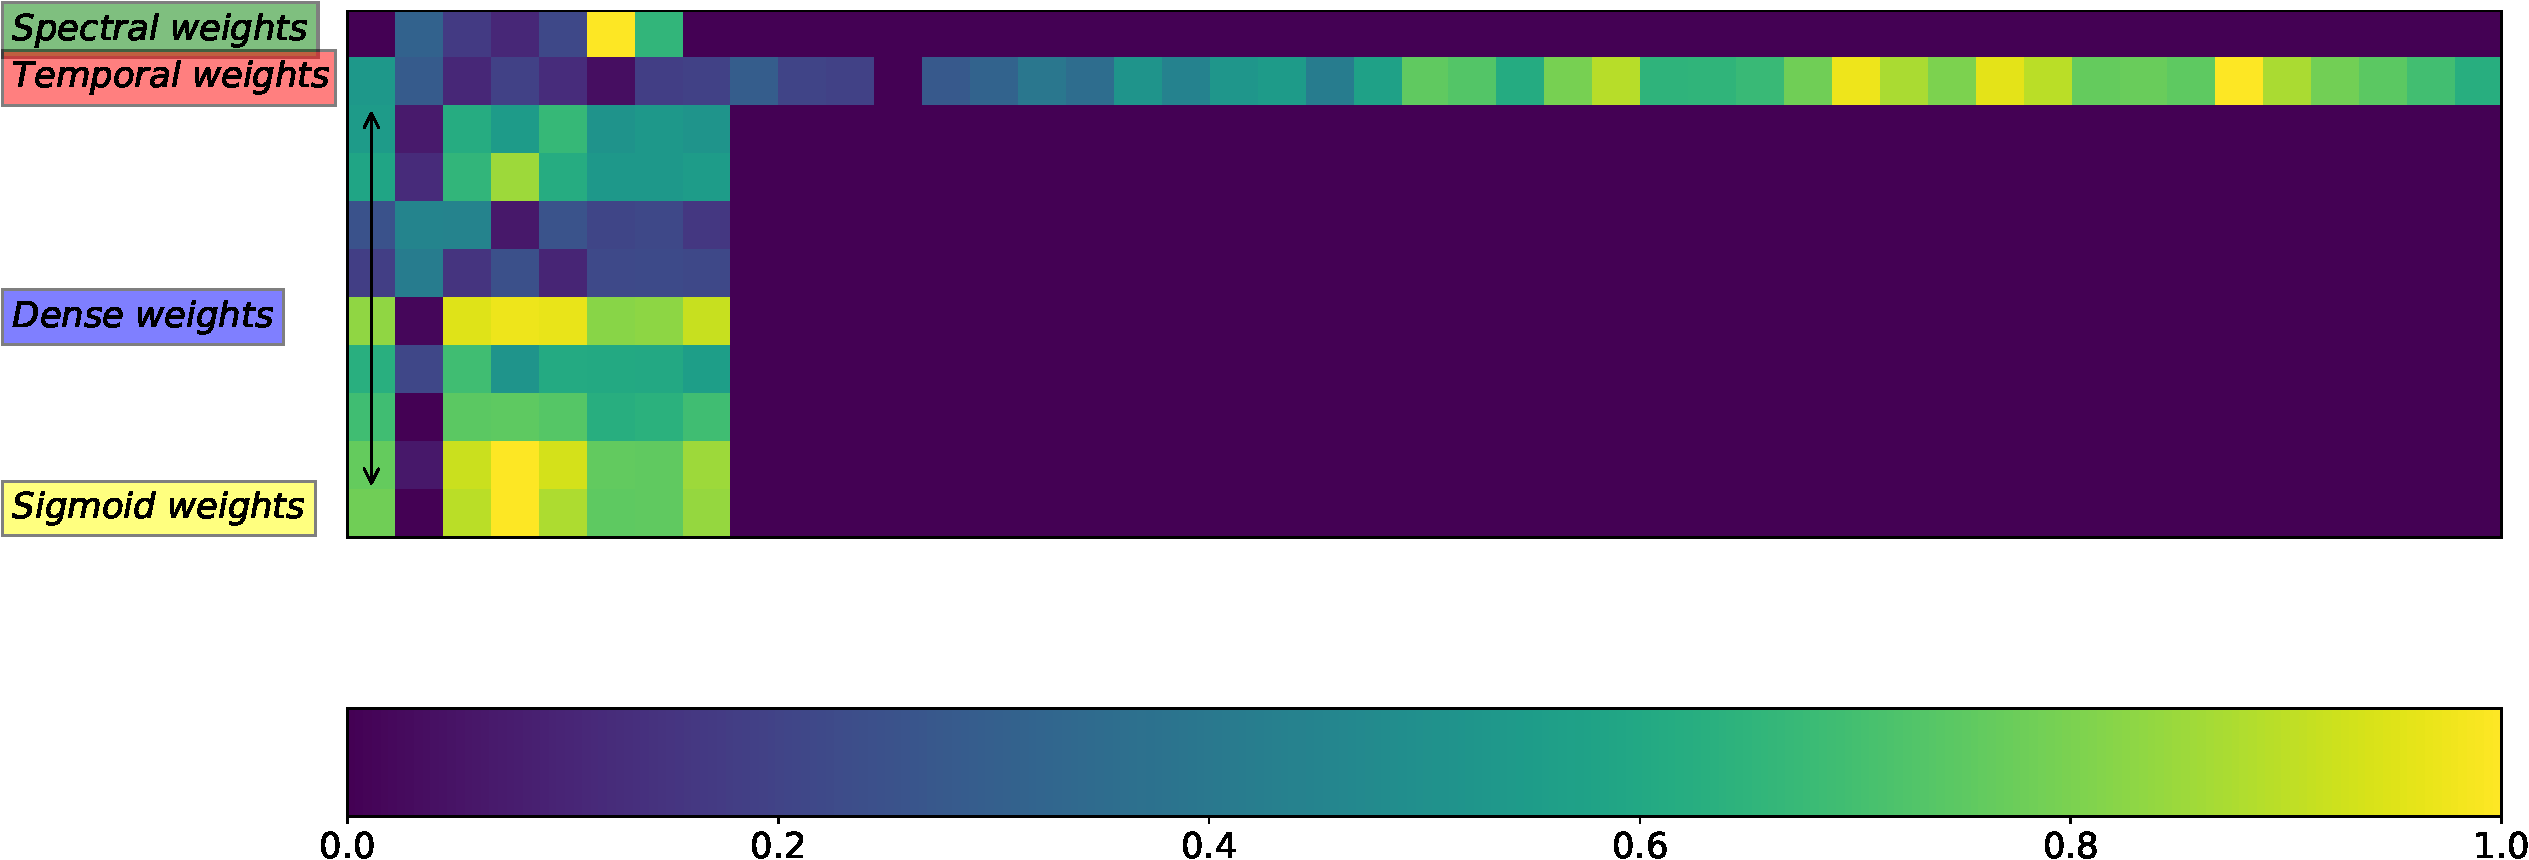
\includegraphics[width=1.0\textwidth]{weights-crop.pdf} 
\caption{The normalized weights associated with a randomly trained model of architecture B. Normalization was performed per layer. There are seven spectral weights and 45 temporal weights associated with the spectral and temporal convolutional layers. The dense layer contains 64 weights and the output layer contains eight weights.}
\label{fig:weights}

\end{figure*}

% \begin{figure*}[h] 
%   \begin{subfigure}[b]{0.5\linewidth}
%     \centering
%     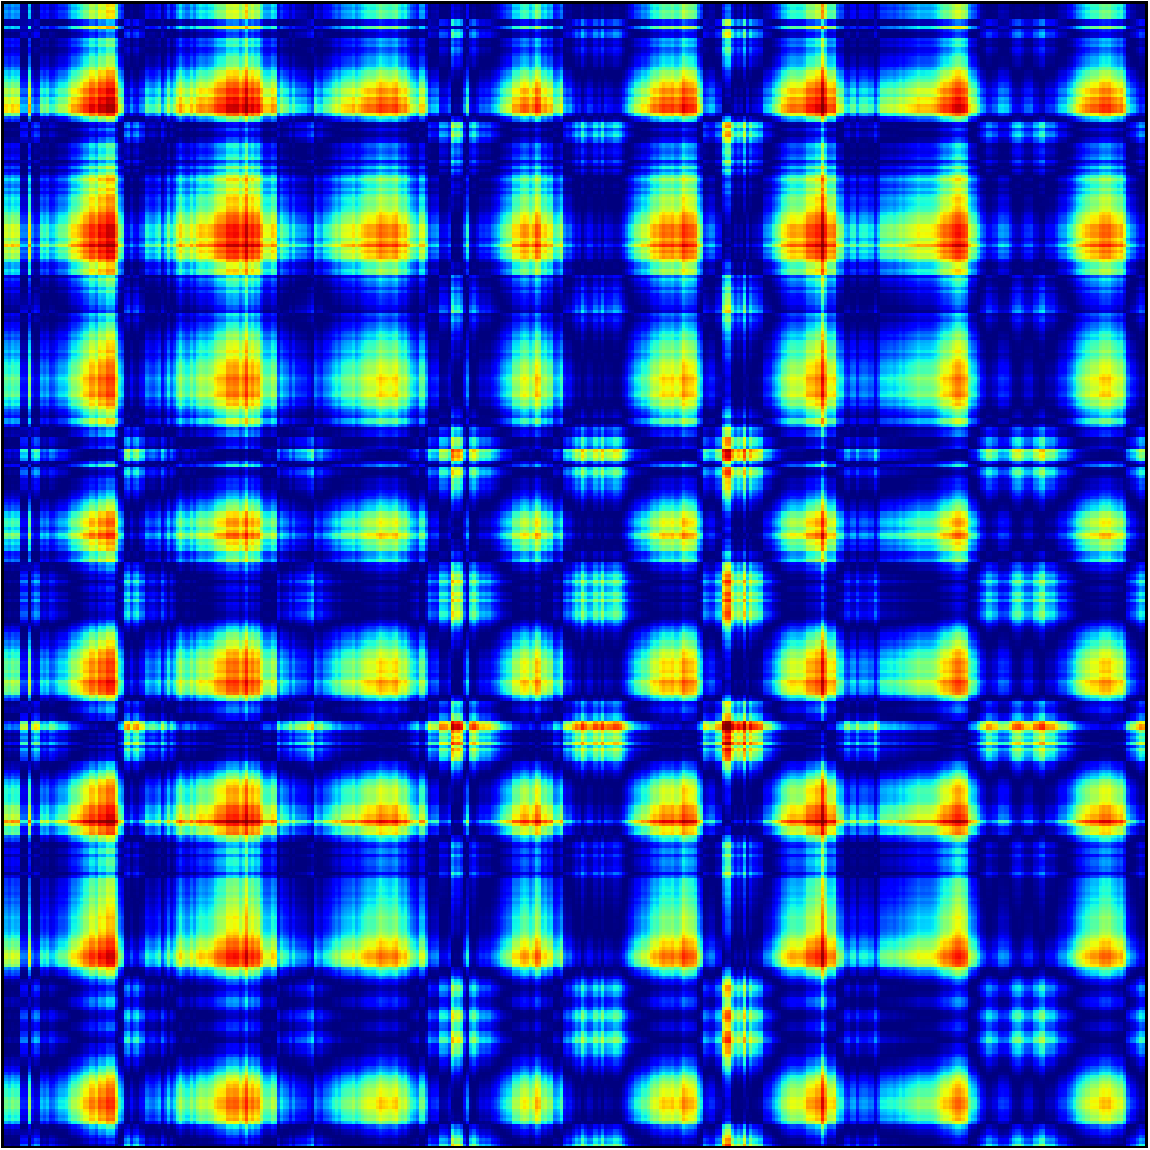
\includegraphics[width=0.89\linewidth]{veg-crop.pdf} 
%     \caption{Vegetation} 
%     \label{fig7:a} 
%     \vspace{6ex}
%   \end{subfigure}%% 
%   \begin{subfigure}[b]{0.5\linewidth}
%     \centering
%     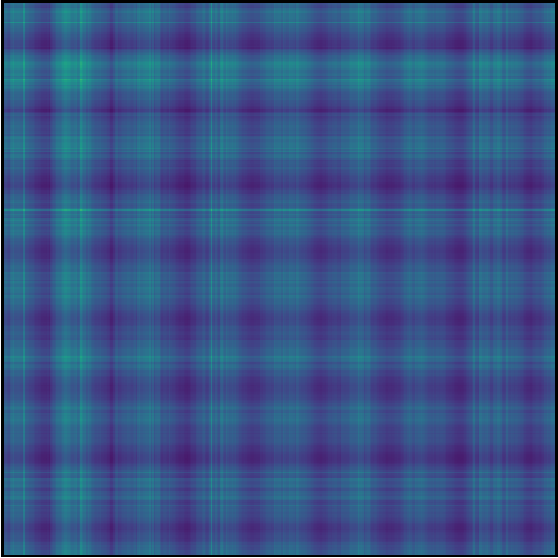
\includegraphics[width=0.89\textwidth]{bwt-crop.pdf} 
%     \caption{Settlement} 
%     \label{fig7:b} 
%     \vspace{6ex}
%     \end{subfigure} 
%     %\vspace{13ex}
%   \begin{subfigure}[b]{0.5\linewidth}
%     \centering
%     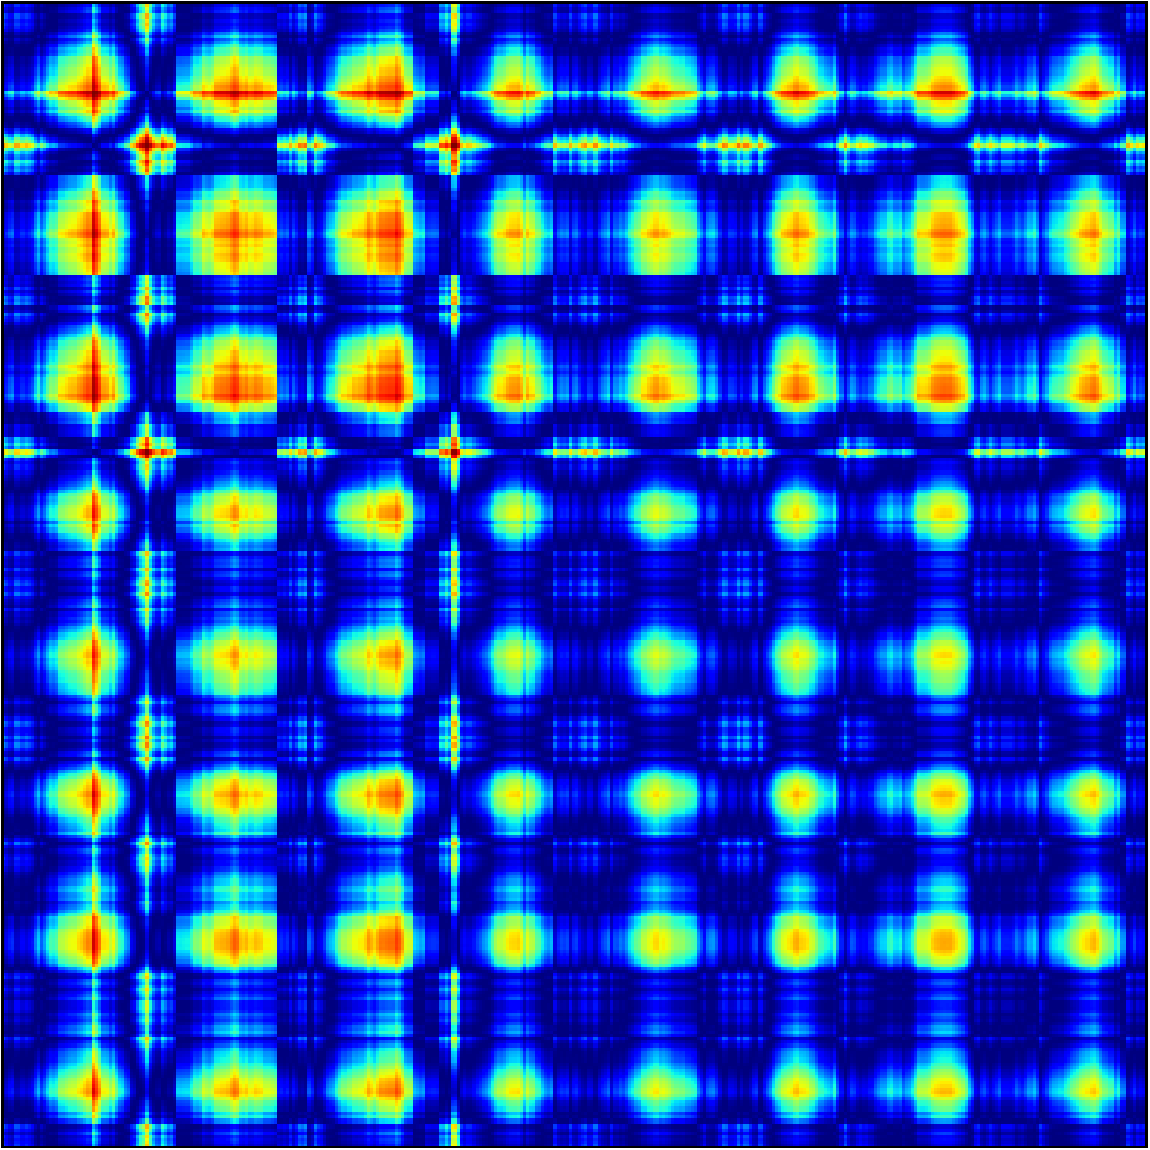
\includegraphics[width=0.89\textwidth]{sim_c-crop.pdf} 
%     \caption{Simulated Change} 
%     \label{fig7:c} 
%   \end{subfigure}%%
%   \begin{subfigure}[b]{0.5\linewidth}
%     \centering
%     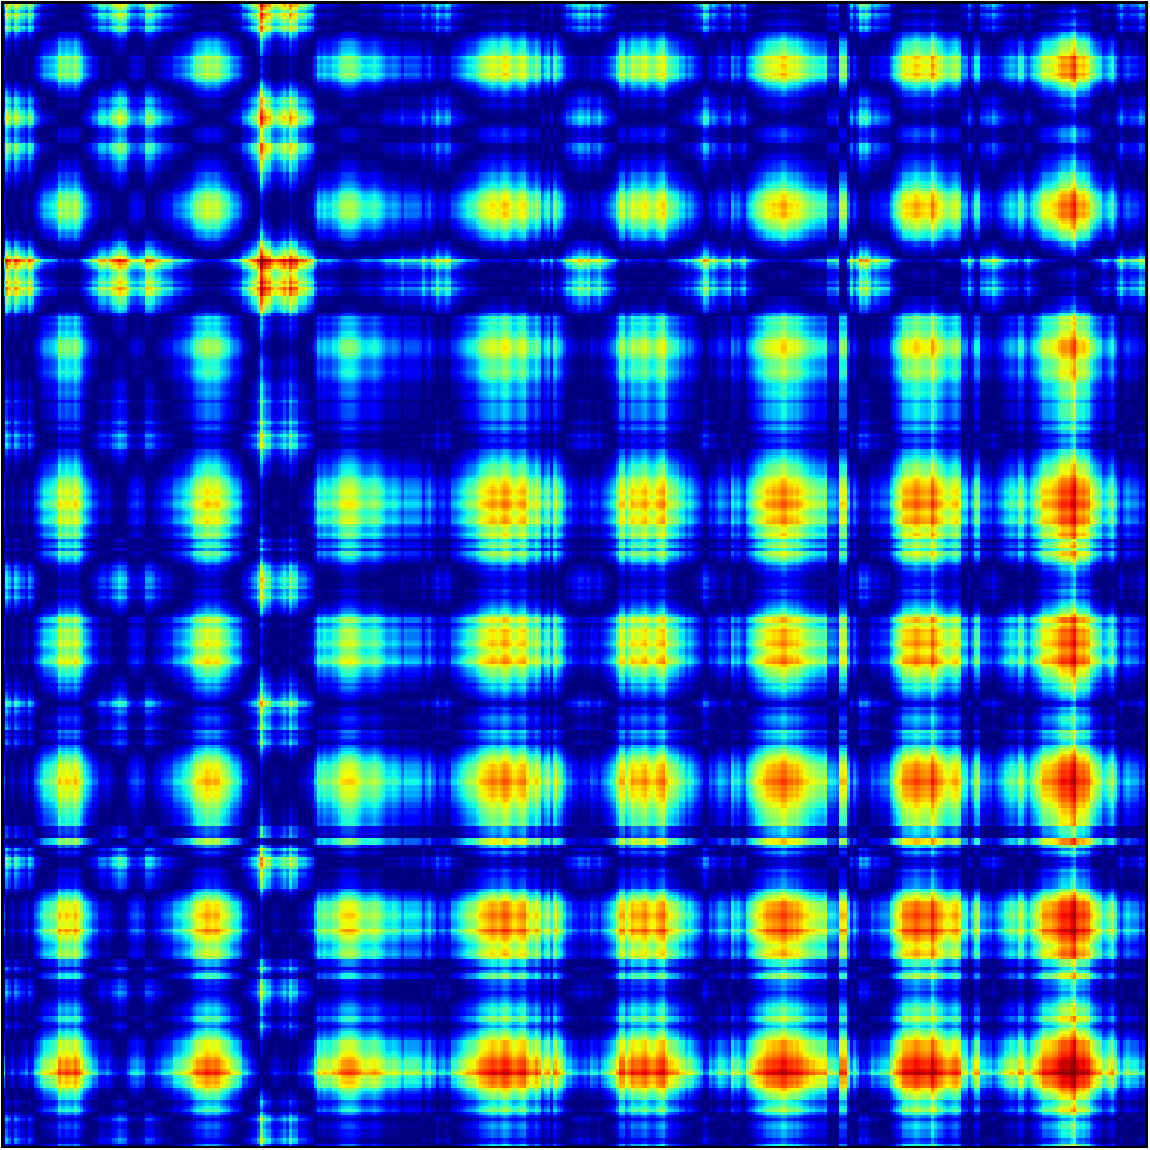
\includegraphics[width=0.89\textwidth]{real_c-crop.pdf} 
%     \caption{Real Change} 
%     \label{fig7:d} 
%   \end{subfigure} 
%   \label{fig:gaf}
%   \caption{The GAF encoding of a random vegetation pixel (top left), a random settlement pixel (top right), a random synthesized changed pixel (bottom left) and a random real change pixel (bottom right) (see Section~\ref{sec:exp}). The GAF transform encodes time-series as images so that the capability of image-based classifiers can be exploited to perform time-series classification (see Section~\ref{sec:GAF}).  The two images in the top panel are visually discernible from one another. The bottom two images are more irregular in nature than the images in the top panel.}
%   \label{fig:gaf}
% \end{figure*}






% To start a new column (but not a new page) and help balance the last-page
% column length use \vfill\pagebreak.
% -------------------------------------------------------------------------

%\section{REFERENCES}
%\label{sec:ref}

%List and number all bibliographical references at the end of the paper.  The references can be numbered in alphabetic order or in order of appearance in the document.  When referring to them in the text, type the corresponding reference number in square brackets as shown at the end of this sentence \cite{C2}.

% References should be produced using the bibtex program from suitable
% BiBTeX files (here: strings, refs, manuals). The IEEEbib.bst bibliography
% style file from IEEE produces unsorted bibliography list.
% -------------------------------------------------------------------------
\bibliographystyle{IEEEbib}
\bibliography{strings,refs}

\end{document}
